\documentclass[tikz, border=2pt]{standalone}

\usepackage{helvet}
\renewcommand{\familydefault}{\sfdefault}

\usepackage[EULERGREEK]{sansmath}
\sansmath
\usetikzlibrary{arrows.meta}

\begin{document}%

\begin{tikzpicture}[line width=2pt]
\tikzset{>={Latex[width=3mm,length=4mm]}}

% grid
\draw[help lines] (-0.5, -5) grid (13, 18);

  \node[inner sep=0pt] (figa) at (5,10.5)
  {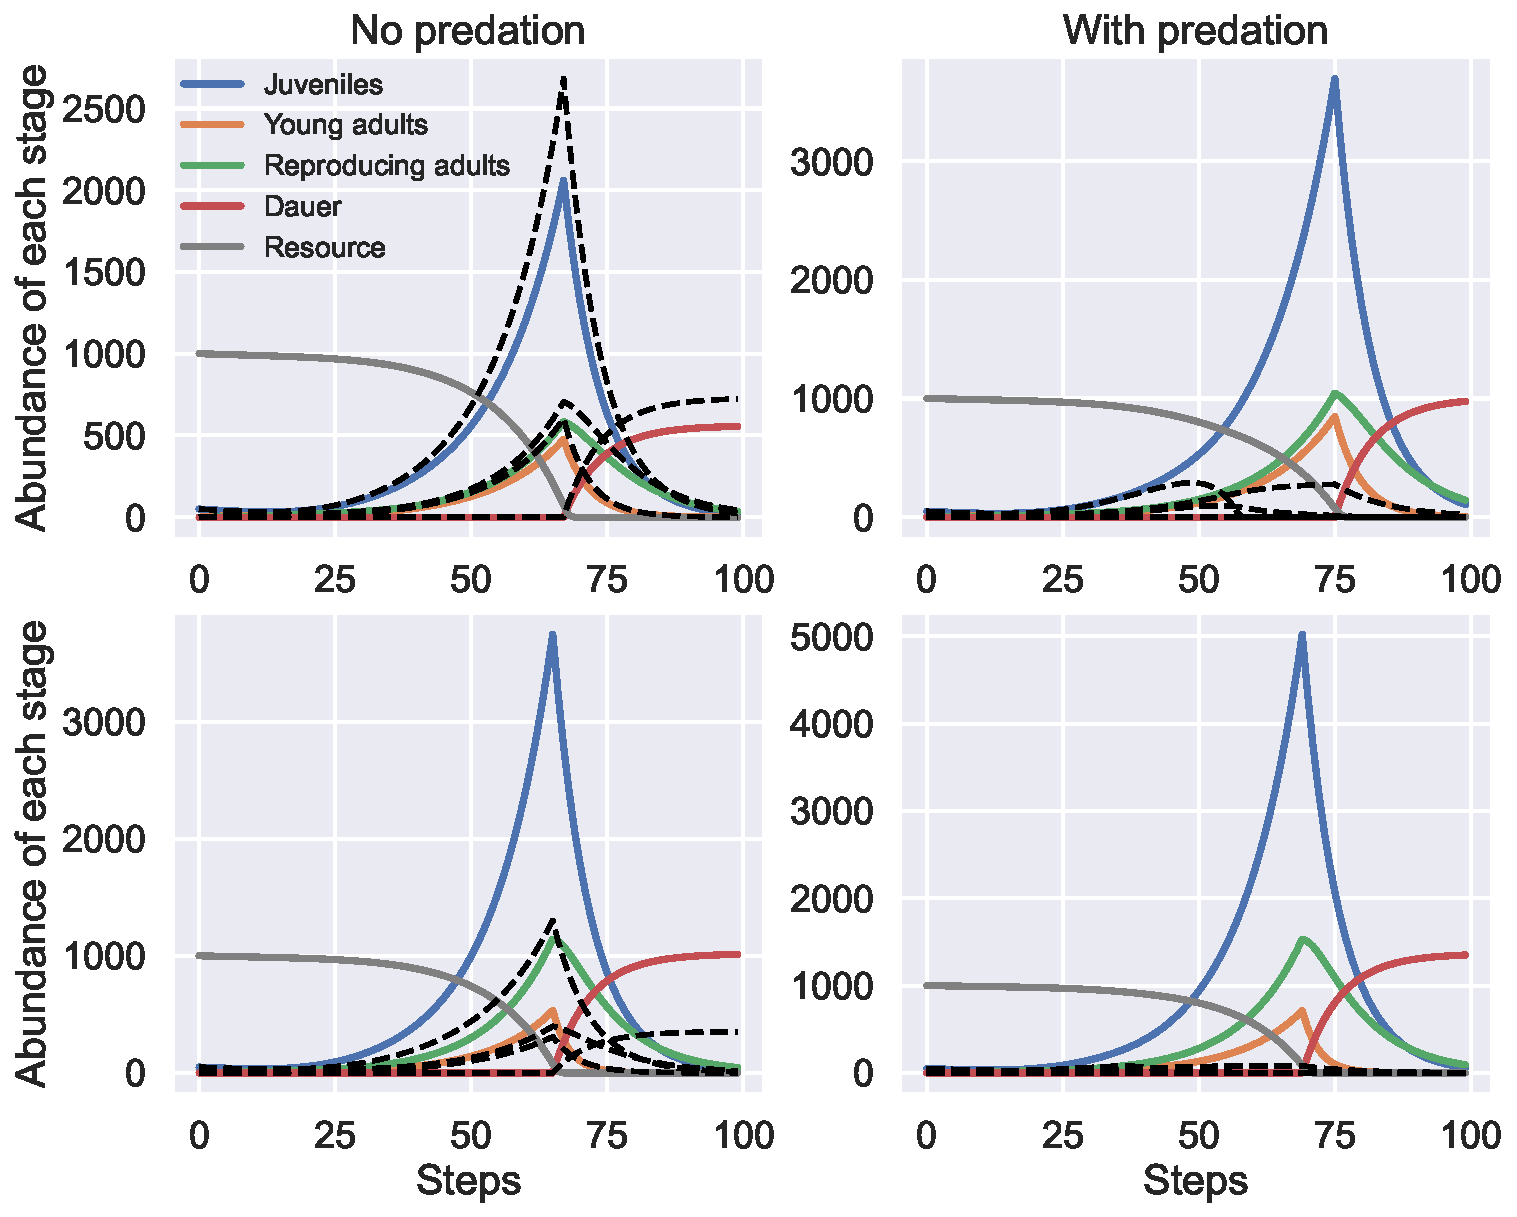
\includegraphics[width=0.8\textwidth]{PopDynamic_with_interaction.pdf}};


  \node[inner sep=0pt] (figa) at (8,4)
  {
\includegraphics[width=0.35\textwidth]{diffusion.pdf}};


  \node[inner sep=0pt] (figa) at (12,12.5)
  {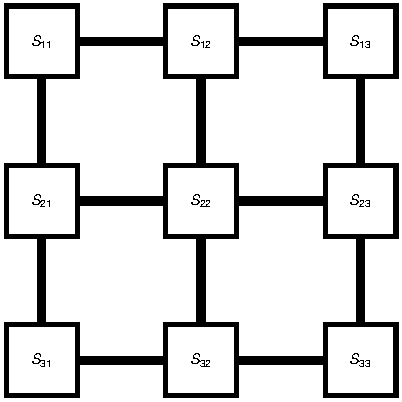
\includegraphics[width=0.28\textwidth]{./tikz_figs/meta_pop.pdf}};


\node at (-0.1,12.5) [draw=white, rectangle, rotate=90] (g1) {\sf \small \emph{E. coli} OP50};

\node at (-0.1,9) [draw=white, rectangle, rotate=90] (g1) {\sf \small \emph{Novosphingobium}};



%labels
\draw (0., 14.8) node{{\Huge\sf\textbf{a}}};

\draw (10.3, 14.8) node{{\Huge\sf\textbf{b}}};

\draw (5.5, 6.3) node{{\Huge\sf\textbf{c}}};

% \draw (0., 11.5) node{{\Huge\sf\textbf{c}}};

% \draw (0., 6.3) node{{\Huge\sf\textbf{d}}};


\end{tikzpicture}


\end{document}